% Standalone replacement for the Experiments and Results section in sn-article (8).tex.
% The structure follows the MOSAIC method chain:
% report-supervision bottleneck -> weak-oracle completion -> section alignment ->
% train-only semantic retrieval and validation-calibrated fusion -> stress tests.

\section{Experiments and Results}
\label{sec:experiments_results}

The experimental programme was organised to mirror the MOSAIC pipeline rather than to list independent analyses. We first quantified the report-supervision bottleneck that motivates weak-oracle learning. We then tested whether pseudo reports contained modality-grounded semantic information beyond label templates, whether section-aware RASA alignment produced a measurable cross-modal semantic organisation, and whether pseudo-report supervision was most useful when real reports were scarce. Only after these mechanism checks did we evaluate the full MOSAIC predictor, which combines the MOSAIC--RASA backbone with a train-only semantic retrieval bank and validation-calibrated logit fusion. Semantic-tag, quality-control, perturbation, leave-one-centre-out, and scalability analyses were used to bound the interpretation of the result rather than to widen the claim.

All analyses used the locked retrospective five-centre cohort and the fixed train/validation/test split of 1,325/284/288 cases. Test labels were used only for final metric computation and bootstrap resampling. Pseudo-report construction, retrieval-bank construction, fusion-weight selection, and operating-threshold selection were restricted to the training and validation protocol described in Methods. Table~\ref{tab:experiment_logic_map} summarises how each result block connects to the corresponding method component.

\begin{table*}[!htbp]
  \centering
  \caption{Experimental logic linking the MOSAIC method components to the result blocks.}
  \label{tab:experiment_logic_map}
  \scriptsize
  \begin{threeparttable}
  \resizebox{\linewidth}{!}{%
  \begin{tabular}{p{3.0cm}p{4.2cm}p{4.4cm}p{4.4cm}}
    \toprule
    \textbf{Result block} & \textbf{Method component being tested} & \textbf{Primary question} & \textbf{Main evidence used in this section} \\
    \midrule
    Cohort and supervision imbalance & Study design and weak-oracle problem formulation & Is there a real report-supervision bottleneck rather than only an image-scale problem? & Five-centre case, image, report, and pseudo-report counts; centre-level report coverage \\
    Weak-oracle report construction & Phase O: LCAD QC-gated completion & Do pseudo reports add modality-grounded semantics beyond class-label templates? & Source comparison, modality support, duplication, masking validation, provider feasibility audit \\
    Section alignment and scarcity & Phase S: RASA section anchors & Do report sections organise multimodal representations and help when real reports are scarce? & Modality-section retrieval, scarcity curve, pseudo-report-augmented surrogate \\
    Held-out risk stratification & Phase A+I+C: train-only retrieval and calibrated fusion & Does the semantic prior improve the locked test predictor over the backbone? & MOSAIC-RASA, retrieval-only, and MOSAIC test metrics; paired bootstrap audit \\
    Claim-boundary audits & Tag retrieval, QC stress testing, perturbation, LOCO, robustness & What does the evidence not establish? & MOSAIC-Tag secondary audit, failure-enriched QC, perturbation matrix, strict LOCO, scalability and stability \\
    \bottomrule
  \end{tabular}%
  }
  \end{threeparttable}
\end{table*}

\FloatBarrier

\subsection{Five-centre cohort and report-supervision bottleneck}
\label{subsec:cohort_results}

The final analytic cohort contained 1,897 multimodal cervical screening cases from five centres, with 129,030 OCT files, 8,561 colposcopy-associated files, and 137,591 total evaluable image files (Table~\ref{tab:baseline_all3000_5cens}). Report availability was much more limited than image availability. Clinician-authored archived reports were available for 744 cases, whereas 1,153 cases had multimodal evidence but no archived report and therefore required weak-oracle pseudo-report supervision if they were to contribute report-level semantic targets.

\begin{table*}[!htbp]
  \centering
  \caption{Five-centre cohort scale and report-supervision availability.}
  \label{tab:baseline_all3000_5cens}
  \scriptsize
  \begin{threeparttable}
  \resizebox{\linewidth}{!}{%
  \begin{tabular}{lrrrrr}
    \toprule
    \textbf{Centre} & \textbf{Cases} & \textbf{OCT images} & \textbf{Colposcopy images} & \textbf{Real reports} & \textbf{Pseudo-report candidates} \\
    \midrule
    Enshi Central Hospital & 406 & 48,504 & 1,233 & 406 & 0 \\
    Jingzhou First People's Hospital & 406 & 12,428 & 2,967 & 334 & 72 \\
    Shiyan People's Hospital & 496 & 14,267 & 1,488 & 0 & 496 \\
    Renmin Hospital of Wuhan University & 89 & 10,680 & 267 & 0 & 89 \\
    Xiangyang Central Hospital & 500 & 43,151 & 2,606 & 4 & 496 \\
    \midrule
    \textbf{Overall} & \textbf{1,897} & \textbf{129,030} & \textbf{8,561} & \textbf{744} & \textbf{1,153} \\
    \bottomrule
  \end{tabular}%
  }
  \begin{tablenotes}[flushleft]
    \footnotesize
    \item Image counts were recomputed from the canonical case manifest. Archived-report status describes source-document availability only and was not used as a model input. The locked test set contained 288 cases.
  \end{tablenotes}
  \end{threeparttable}
\end{table*}

\begin{figure}[!htbp]
  \centering
  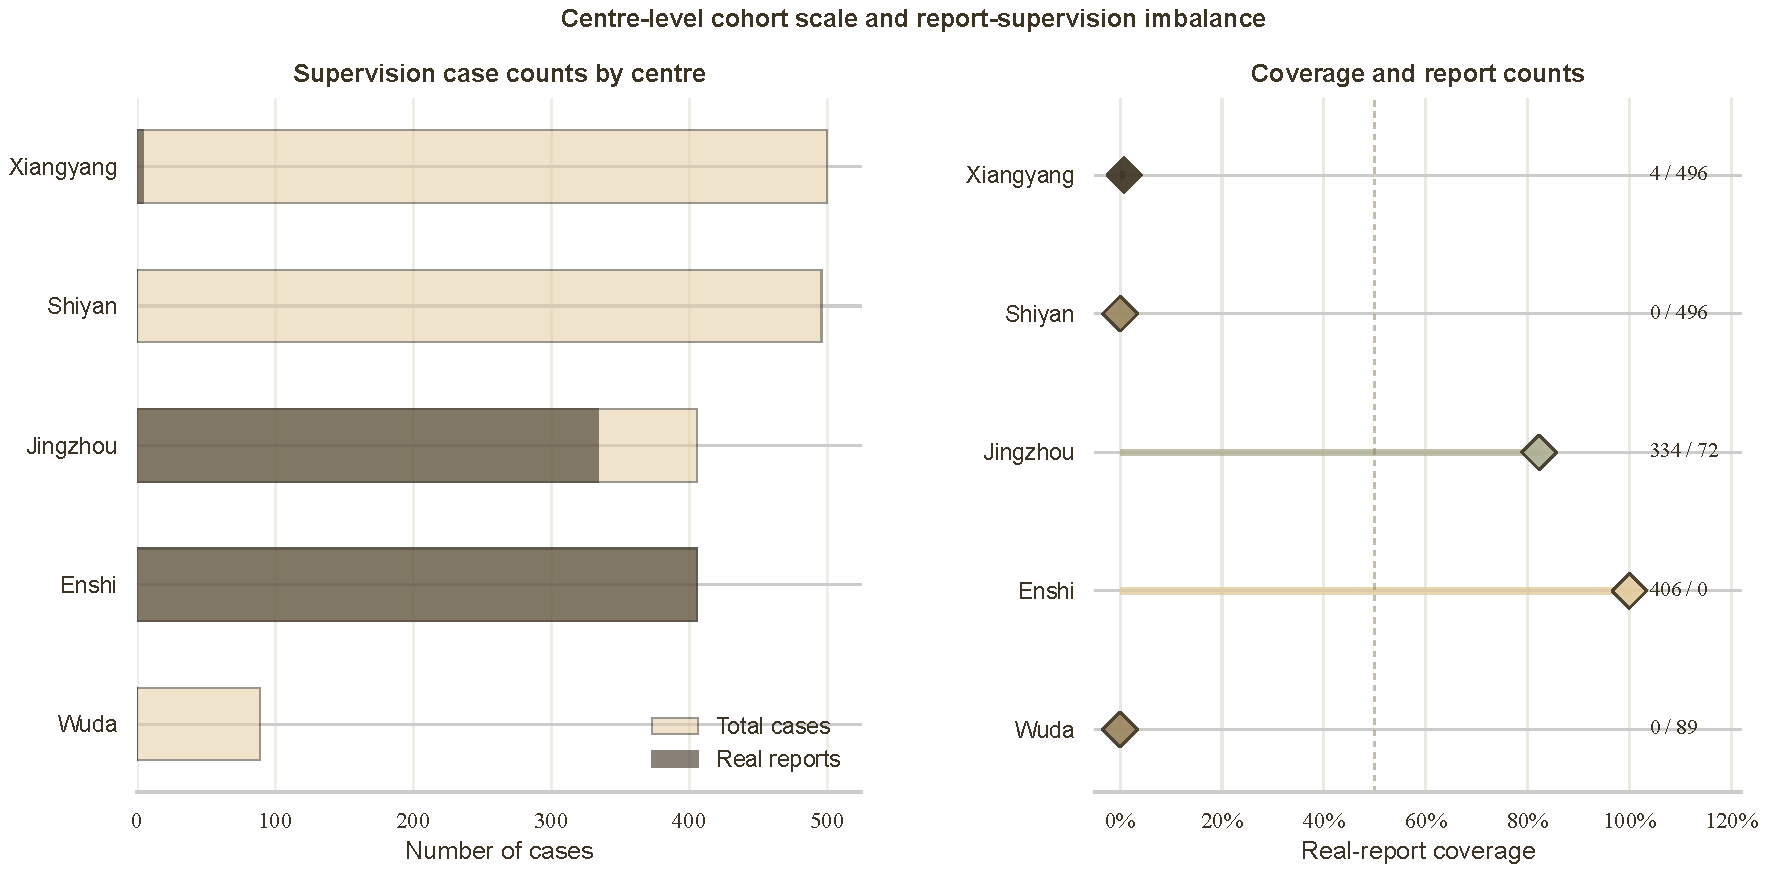
\includegraphics[width=\linewidth]{final_Fig/Figure2_centre_supervision_catplot.pdf}
  \caption{Centre-stratified report-supervision imbalance. Case counts and image volume were large across centres, but report coverage was highly uneven, motivating the weak-oracle formulation rather than a complete-case-only analysis.}
  \label{fig:centre_supervision}
\end{figure}

The missingness pattern was strongly centre-dependent: Enshi retained reports for all 406 cases, Jingzhou for 334 of 406 cases, Xiangyang for only 4 of 500 cases, and Wuhan and Shiyan had no centre-wide report archive. This pattern defines the central experimental setting. MOSAIC does not treat generated text as physician-authored documentation; it uses QC-gated pseudo reports as weak semantic scaffolds for cases that would otherwise lack report-level supervision.

\FloatBarrier

\subsection{Weak-oracle pseudo reports carry more signal than label templates}
\label{subsec:pseudo_report_results}

The next experiment tested whether pseudo reports supplied modality-grounded semantic content or merely restated class labels. A label-template source produced schema-complete reports, but it had no modality support and a high maximum duplicate fraction of 0.867 (Table~\ref{tab:pseudo_source_comparison}). In contrast, the rule-based and local embedding-assisted LLM sources both achieved modality-support rates of 1.000, higher label-consistency values, and substantially lower duplicate fractions. This comparison establishes the negative control for Phase O: a valid schema alone is not sufficient; report sections must remain connected to OCT, colposcopy, and clinical evidence.

\begin{table*}[!htbp]
  \centering
  \caption{Structured pseudo-report source comparison.}
  \label{tab:pseudo_source_comparison}
  \scriptsize
  \begin{threeparttable}
  \resizebox{\linewidth}{!}{%
  \begin{tabular}{lrrrrr}
    \toprule
    \textbf{Source} & \textbf{$n$} & \textbf{Label consistency} & \textbf{Modality support} & \textbf{Unique text} & \textbf{Duplicate fraction} \\
    \midrule
    Label template & 180 & 0.567 & 0.000 & 0.011 & 0.867 \\
    Rule-based & 180 & \textbf{0.628} & \textbf{1.000} & \textbf{0.194} & \textbf{0.200} \\
    Local embedding-assisted LLM & 180 & \textbf{0.628} & \textbf{1.000} & 0.156 & 0.261 \\
    \bottomrule
  \end{tabular}%
  }
  \begin{tablenotes}[flushleft]
    \footnotesize
    \item All sources produced schema-complete reports, so the complete-rate column was omitted. Pseudo reports are used as weighted semantic supervision, not as clinical ground truth.
  \end{tablenotes}
  \end{threeparttable}
\end{table*}

\begin{figure}[!htbp]
  \centering
  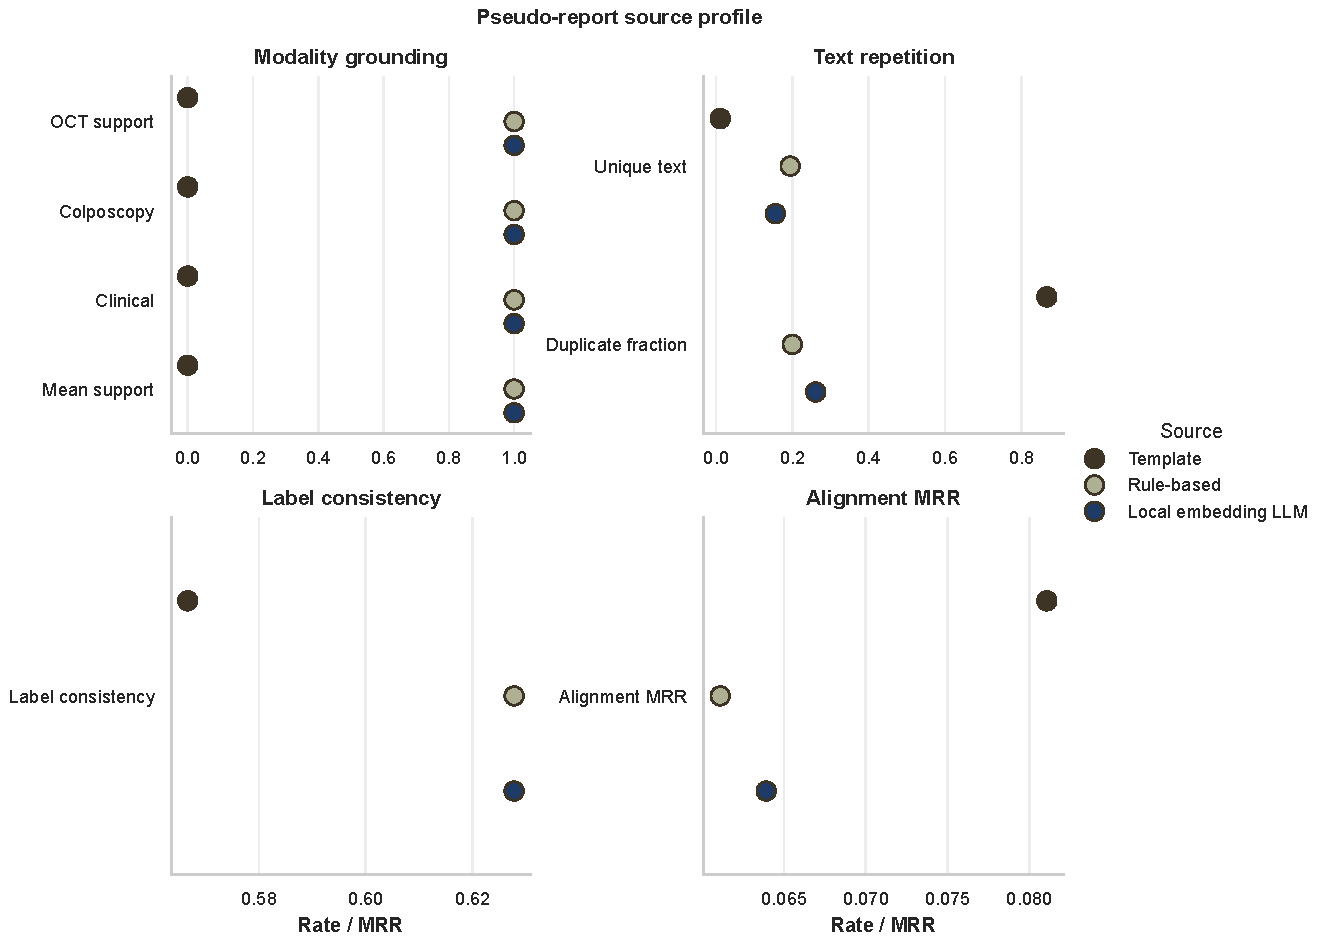
\includegraphics[width=\linewidth]{final_Fig/Figure_theme1_pseudo_report_source_comparison.pdf}
  \caption{Structured pseudo-report source comparison. The label-template control shows that schema completion alone can be repetitive and ungrounded, whereas rule-based and local embedding-assisted LLM reports preserve modality-specific support.}
  \label{fig:pseudo_source_comparison}
\end{figure}

External provider analyses were treated as an auxiliary implementation audit, not as the default MOSAIC training source. Only de-identified structured evidence was sent to providers; raw images, image paths, patient names, internal identifiers, hospital identifiers, and directly identifying information were not transmitted. In the extended 100-case API cohort, GPT-5.5 produced 100 schema-valid structured reports, with section completeness 0.810, modality support 0.810, contradiction rate 0.050, hallucination rate 0.000, mean latency 11.39 seconds per case, and estimated cost of US\$27.73 per 1,000 cases. Pilot cohorts for Qwen-Plus, GLM-4.7-Flash, and Gemini-3.1-Pro are therefore reported as feasibility and operational-reliability evidence rather than as definitive provider rankings.

\FloatBarrier

\subsection{Section-aware alignment and scarcity analyses support the weak-oracle mechanism}
\label{subsec:alignment_scarcity_results}

Phase S was evaluated by asking whether modality-specific embeddings retrieved their corresponding report sections. OCT embeddings queried \texttt{oct\_findings}, colposcopy embeddings queried \texttt{colposcopy\_findings}, clinical embeddings queried \texttt{clinical\_context}, and fused representations queried \texttt{impression}. The MOSAIC--RASA backbone achieved macro MRR 0.051, compared with 0.021 after removing section alignment and 0.022 for simple concatenation fusion (Table~\ref{tab:theme1_alignment_ablation}). The absolute retrieval values were modest, so the finding is interpreted as relative section organisation under a stringent retrieval audit rather than as high-fidelity free-form semantic retrieval.

\begin{table*}[!htbp]
  \centering
  \caption{Direct RASA alignment ablation using modality-section retrieval.}
  \label{tab:theme1_alignment_ablation}
  \scriptsize
  \begin{threeparttable}
  \resizebox{\linewidth}{!}{%
  \begin{tabular}{lrrrr}
    \toprule
    \textbf{Model} & \textbf{Recall@1} & \textbf{Recall@5} & \textbf{Macro MRR} & \textbf{Positive cosine} \\
    \midrule
    Real-report only & \textbf{0.0182} & 0.0642 & \textbf{0.057} & \textbf{0.984} \\
    Pseudo-augmented LCAD & 0.0139 & \textbf{0.0729} & 0.055 & \textbf{0.984} \\
    MOSAIC--RASA backbone & 0.0148 & 0.0608 & 0.051 & \textbf{0.984} \\
    No section alignment & 0.0052 & 0.0139 & 0.021 & 0.013 \\
    Simple concatenation fusion & 0.0035 & 0.0182 & 0.022 & 0.021 \\
    \bottomrule
  \end{tabular}%
  }
  \end{threeparttable}
\end{table*}

\begin{figure*}[!htbp]
  \centering
  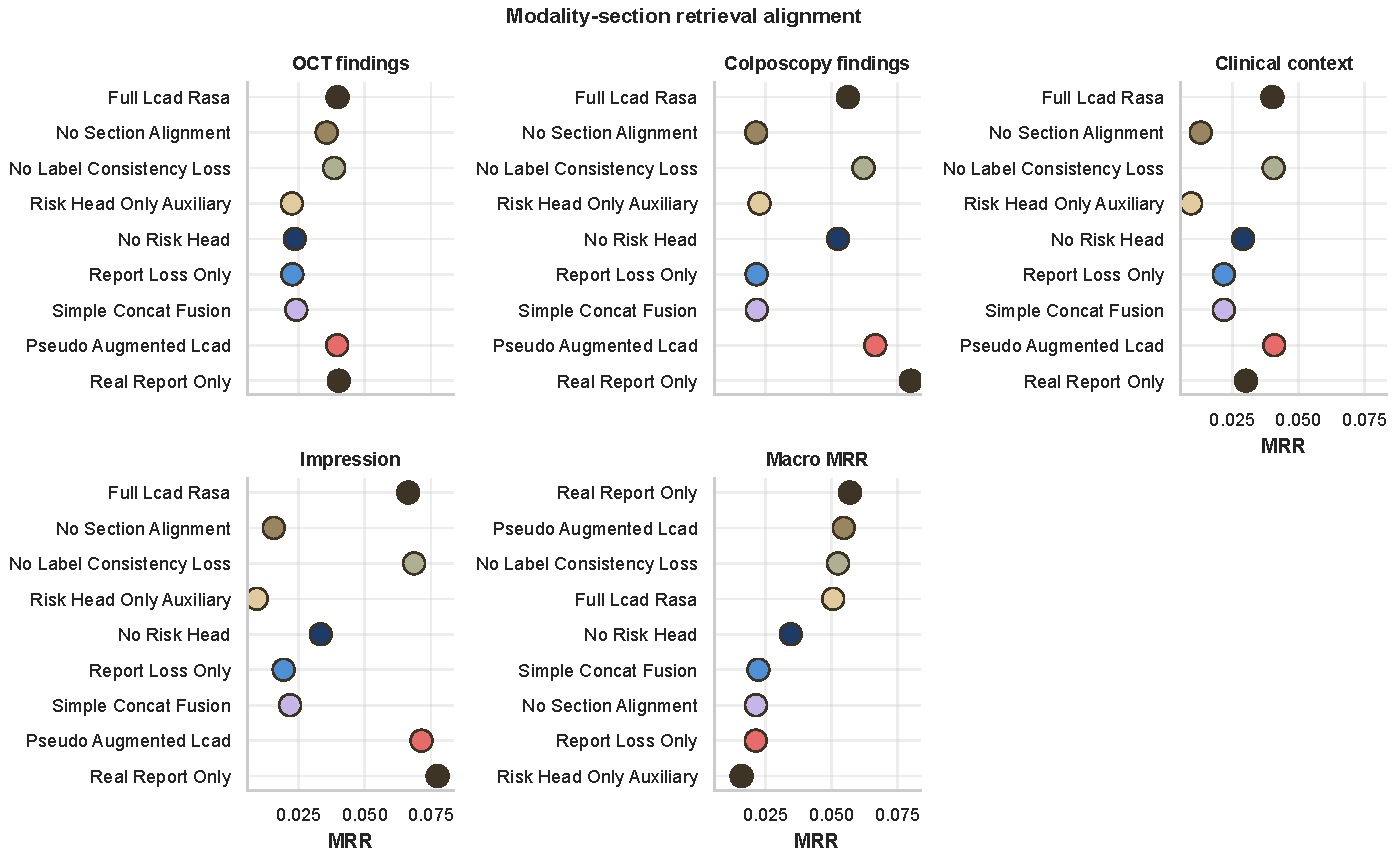
\includegraphics[width=0.49\linewidth]{final_Fig/Figure_theme1_alignment_retrieval_mrr.pdf}
  \hfill
  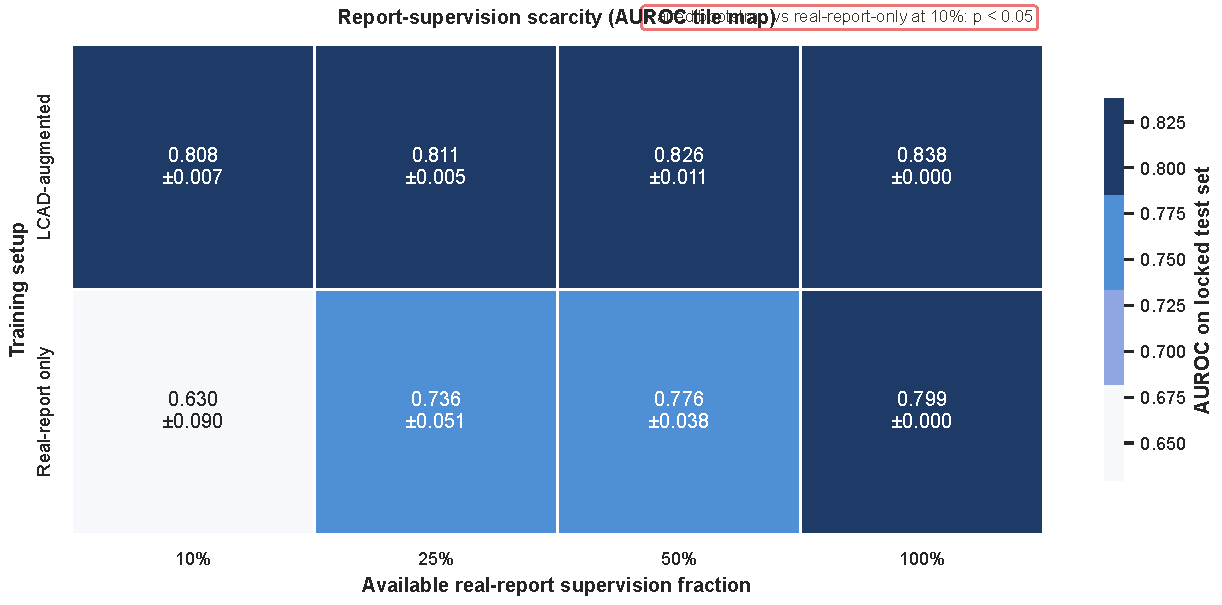
\includegraphics[width=0.49\linewidth]{final_Fig/Figure_theme1_report_supervision_scarcity_curve.pdf}
  \caption{Mechanism analyses for section-aware weak supervision. Left: modality-section retrieval tests whether RASA aligns each modality with its corresponding report section. Right: the report-scarcity curve tests whether pseudo-report augmentation is most useful when real report supervision is limited.}
  \label{fig:alignment_and_scarcity}
\end{figure*}

The scarcity experiment tested the practical consequence of this alignment signal. When only 10\% of real-report supervision was retained, the LCAD-augmented surrogate achieved AUROC 0.808 and F1 0.500, compared with AUROC 0.630 and F1 0.316 for the real-report-only surrogate (Table~\ref{tab:scarcity_curve}). The gap narrowed but persisted at full real-report availability. This pattern is consistent with the intended use case of MOSAIC: pseudo reports are most useful when image and clinical evidence are available at scale but report-level supervision is sparse.

\begin{table*}[!htbp]
  \centering
  \caption{Report-supervision scarcity curve using a lightweight downstream surrogate.}
  \label{tab:scarcity_curve}
  \scriptsize
  \begin{threeparttable}
  \resizebox{\linewidth}{!}{%
  \begin{tabular}{llrrrrr}
    \toprule
    \textbf{Real-report fraction} & \textbf{Setup} & \textbf{Train $n$} & \textbf{Real $n$} & \textbf{Pseudo $n$} & \textbf{AUROC} & \textbf{F1} \\
    \midrule
    1.00 & LCAD-augmented surrogate & 1,325 & 520 & 805 & \textbf{0.838} & \textbf{0.542} \\
    1.00 & Real-report-only surrogate & 520 & 520 & 0 & 0.799 & 0.471 \\
    0.50 & LCAD-augmented surrogate & 1,065 & 260 & 805 & \textbf{0.826} & \textbf{0.526} \\
    0.50 & Real-report-only surrogate & 260 & 260 & 0 & 0.776 & 0.442 \\
    0.25 & LCAD-augmented surrogate & 935 & 130 & 805 & \textbf{0.811} & \textbf{0.485} \\
    0.25 & Real-report-only surrogate & 130 & 130 & 0 & 0.736 & 0.383 \\
    0.10 & LCAD-augmented surrogate & 857 & 52 & 805 & \textbf{0.808} & \textbf{0.500} \\
    0.10 & Real-report-only surrogate & 52 & 52 & 0 & 0.630 & 0.316 \\
    \bottomrule
  \end{tabular}%
  }
  \end{threeparttable}
\end{table*}

\FloatBarrier

\subsection{Train-only semantic retrieval improves locked held-out risk stratification}
\label{subsec:mosaic_main_results}

The full MOSAIC predictor adds the Phase A+I+C semantic prior to the MOSAIC--RASA backbone. The retrieval bank contained training-derived cervical section entities only; validation and test labels were excluded from bank construction. On the locked held-out test set (\(n=288\)), the MOSAIC--RASA backbone achieved AUROC 0.856, AUPRC 0.662, and F1 0.519 (Table~\ref{tab:mosaic_main}). Semantic retrieval alone was informative but insufficient as a standalone predictor, with AUROC 0.774 and F1 0.585. After validation-calibrated logit fusion (\(\alpha=0.31\)) and a validation-selected threshold of 0.50, MOSAIC achieved AUROC 0.908, AUPRC 0.741, F1 0.736, sensitivity 0.727, precision 0.744, and balanced accuracy 0.841.

\begin{table*}[!htbp]
  \centering
  \caption{Locked held-out test performance of the MOSAIC semantic-prior pipeline.}
  \label{tab:mosaic_main}
  \scriptsize
  \begin{threeparttable}
  \resizebox{\linewidth}{!}{%
  \begin{tabular}{lrrrrrrr}
    \toprule
    \textbf{Method} & \textbf{AUROC} & \textbf{AUPRC} & \textbf{F1} & \textbf{Sensitivity} & \textbf{Precision} & \textbf{Balanced accuracy} & \textbf{Threshold} \\
    \midrule
    MOSAIC--RASA backbone & 0.856 & 0.662 & 0.519 & 0.636 & 0.438 & 0.744 & 0.39 \\
    Semantic retrieval only & 0.774 & 0.589 & 0.585 & 0.545 & 0.632 & 0.744 & 0.67 \\
    \textbf{MOSAIC} & \textbf{0.908} & \textbf{0.741} & \textbf{0.736} & \textbf{0.727} & \textbf{0.744} & \textbf{0.841} & 0.50 \\
    \bottomrule
  \end{tabular}%
  }
  \begin{tablenotes}[flushleft]
    \footnotesize
    \item The semantic retrieval bank was built from the training split only. The fusion weight and threshold were selected on the validation split and locked before test evaluation.
  \end{tablenotes}
  \end{threeparttable}
\end{table*}

\begin{figure}[!htbp]
  \centering
  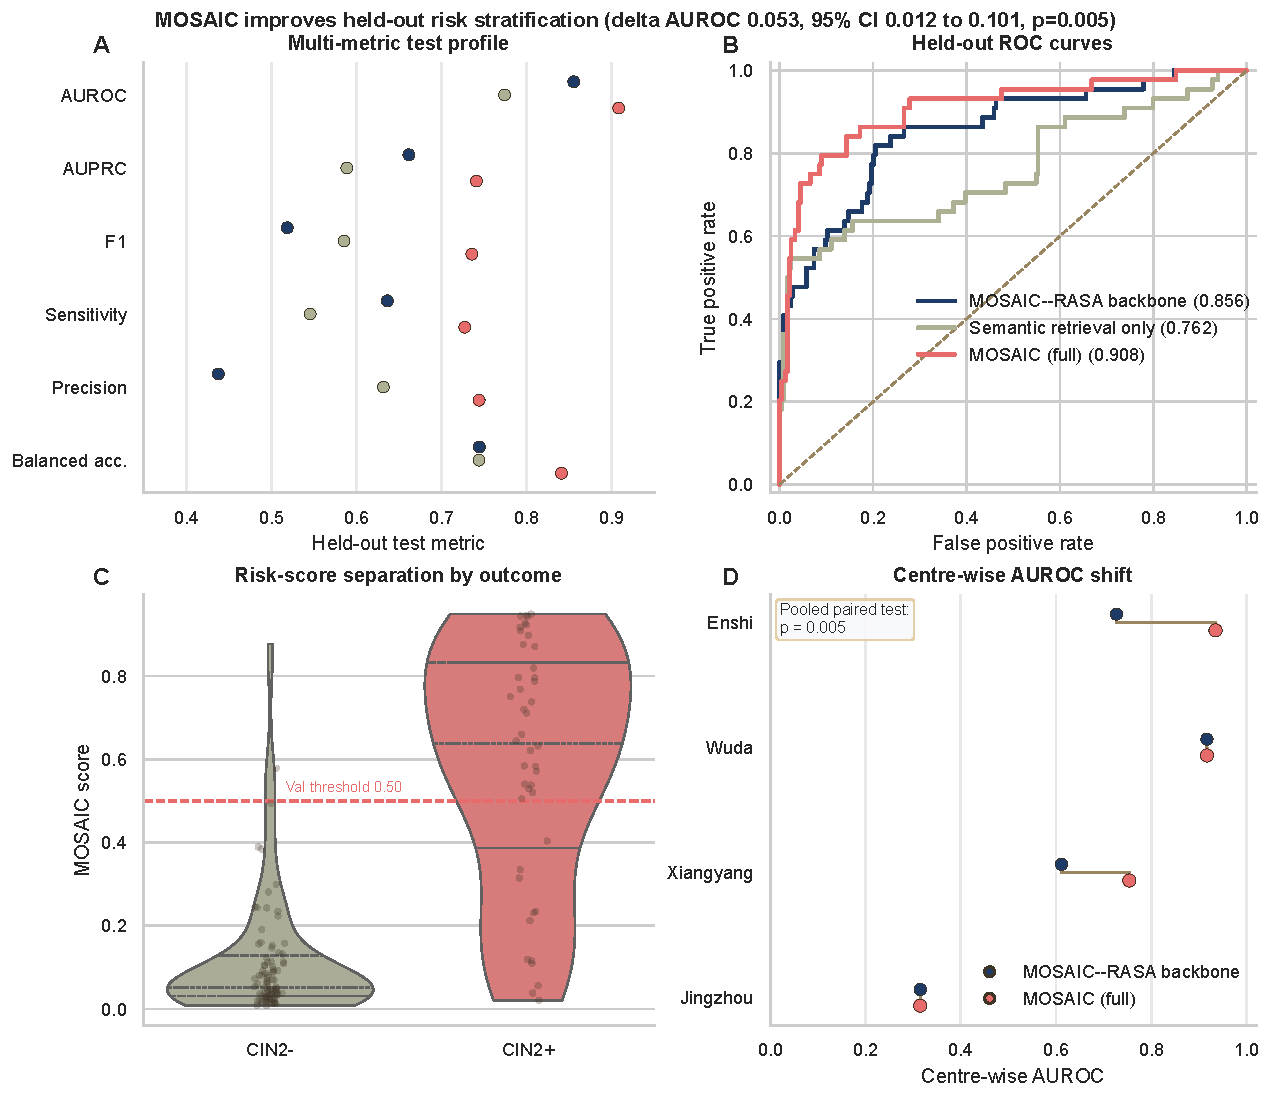
\includegraphics[width=\linewidth]{final_Fig/Figure_mosaic_performance_summary.pdf}
  \caption{Primary MOSAIC held-out performance. The figure summarises the backbone, retrieval-only prior, and fused MOSAIC predictor, including discrimination, score separation, and centre-wise AUROC shifts.}
  \label{fig:mosaic_performance_summary}
\end{figure}

The paired bootstrap audit supports the incremental value of retrieval-calibrated semantic priors over the backbone: MOSAIC improved AUROC by 0.053 over MOSAIC--RASA (95\% CI, 0.012--0.101; two-sided \(p=0.005\); 2,000 resamples). This result should be read as evidence that train-only semantic memory contributes to risk inference under the locked protocol, not as evidence of clinical deployment readiness.

\FloatBarrier

\subsection{Same-split baseline comparison calibrates the strength of the claim}
\label{subsec:external_baseline_results}

The same locked split was used to compare MOSAIC with clinical-only, image-only, late-fusion, cross-attention, and contrastive multimodal baselines. MOSAIC had the highest AUROC point estimate (0.908; 95\% CI, 0.845--0.957), followed by a CLIP-style contrastive multimodal baseline (0.888; 95\% CI, 0.821--0.942) and clinical-only HistGradientBoosting (0.862; 95\% CI, 0.798--0.918) (Table~\ref{tab:external_baselines}). The backbone alone did not dominate the contrastive baseline, so the appropriate primary comparison is the complete MOSAIC pipeline rather than MOSAIC--RASA by itself.

\begin{table*}[!htbp]
  \centering
  \caption{Same-split comparison with external baselines on the locked held-out test set.}
  \label{tab:external_baselines}
  \scriptsize
  \begin{threeparttable}
  \resizebox{\linewidth}{!}{%
  \begin{tabular}{lrrr}
    \toprule
    \textbf{Model} & \textbf{AUROC [95\% CI]} & \textbf{F1 [95\% CI]} & \textbf{Threshold} \\
    \midrule
    \textbf{MOSAIC} & \textbf{0.908 [0.845, 0.957]} & \textbf{0.736 [0.620, 0.830]} & 0.50 \\
    CLIP-style contrastive multimodal baseline & 0.888 [0.821, 0.942] & 0.640 [0.500, 0.753] & 0.79 \\
    Clinical-only HistGradientBoosting & 0.862 [0.798, 0.918] & 0.632 [0.507, 0.741] & 0.68 \\
    MOSAIC--RASA backbone & 0.856 [0.782, 0.915] & 0.519 [0.411, 0.667] & 0.39 \\
    Cross-attention multimodal transformer & 0.847 [0.776, 0.908] & 0.522 [0.385, 0.636] & 0.65 \\
    Clinical-only logistic regression & 0.830 [0.760, 0.889] & 0.557 [0.430, 0.673] & 0.63 \\
    Colposcopy-only embedding MLP & 0.827 [0.756, 0.890] & 0.510 [0.381, 0.627] & 0.74 \\
    Late-fusion MLP & 0.824 [0.750, 0.891] & 0.486 [0.333, 0.625] & 0.77 \\
    OCT-only embedding MLP & 0.786 [0.708, 0.861] & 0.494 [0.344, 0.622] & 0.68 \\
    \bottomrule
  \end{tabular}%
  }
  \begin{tablenotes}[flushleft]
    \footnotesize
    \item All rows used the same train/validation/test split, validation-selected threshold rule, held-out test set, and bootstrap confidence-interval protocol.
  \end{tablenotes}
  \end{threeparttable}
\end{table*}

\begin{figure}[!htbp]
  \centering
  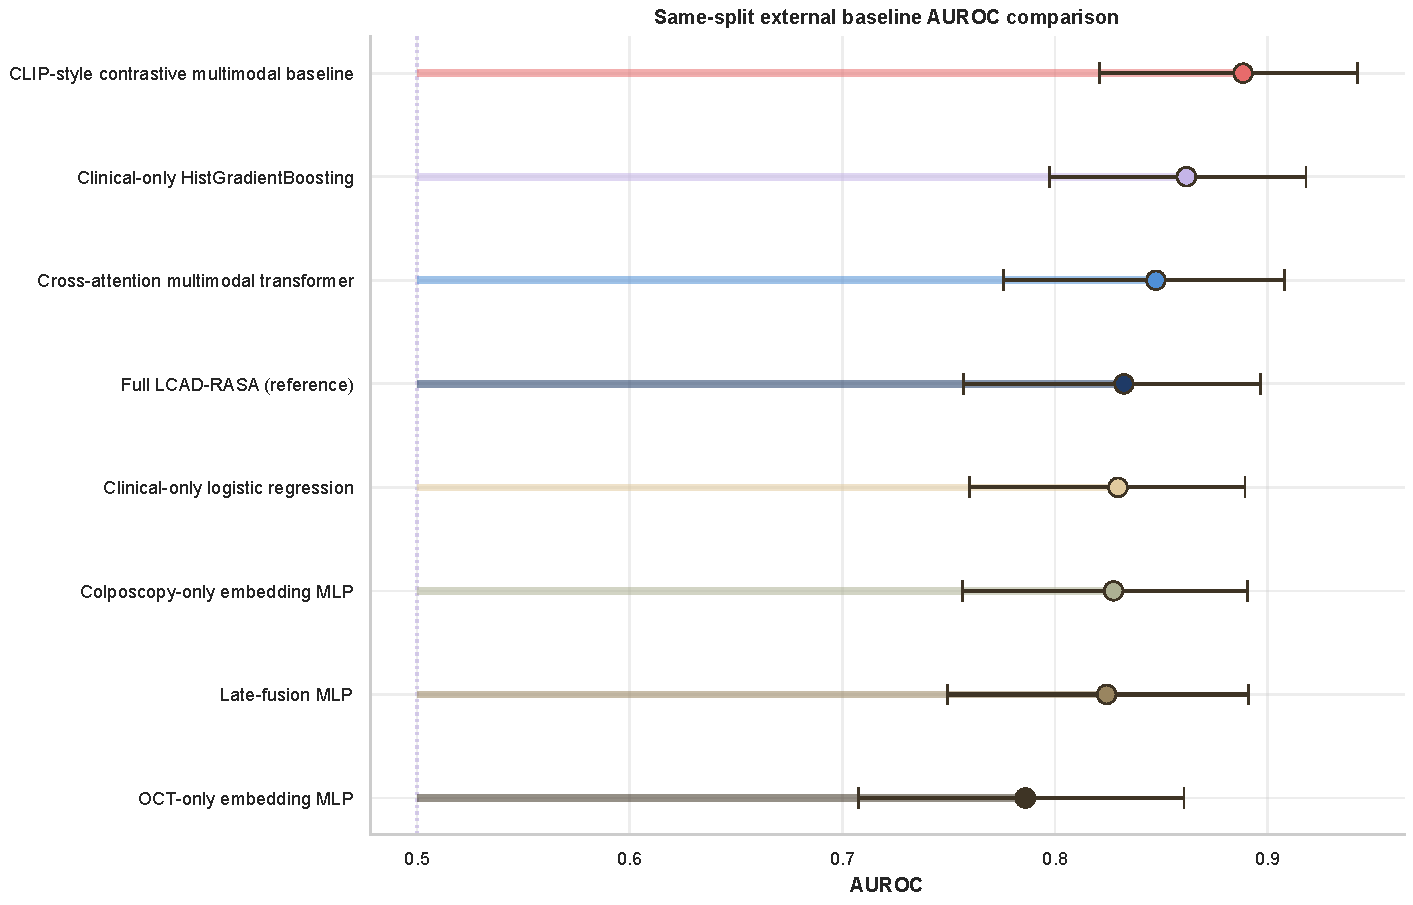
\includegraphics[width=\linewidth]{final_Fig/Figure_external_baselines_auc_forest.pdf}
  \caption{Same-split AUROC comparison against external baselines. Intervals denote bootstrap 95\% confidence intervals on the locked held-out test set.}
  \label{fig:external_baselines_auc}
\end{figure}

The paired comparisons further calibrate the claim (Table~\ref{tab:full_mosaic_paired_bootstrap}). MOSAIC exceeded the CLIP-style contrastive baseline by point estimate, but the paired AUROC interval crossed zero (\(\Delta\)AUROC 0.020; 95\% CI, -0.019--0.065; \(p=0.355\)). Therefore, the manuscript claim is not universal superiority over all multimodal baselines. The supported claim is narrower: under the locked retrospective protocol, incomplete report supervision can be converted into train-only semantic priors that improve MOSAIC over its own backbone and remain competitive with strong same-split multimodal alternatives.

\begin{table*}[!htbp]
  \centering
  \caption{Paired-bootstrap comparison of MOSAIC with same-split comparators. Positive deltas favour MOSAIC.}
  \label{tab:full_mosaic_paired_bootstrap}
  \scriptsize
  \begin{threeparttable}
  \resizebox{\linewidth}{!}{%
  \begin{tabular}{lrrrr}
    \toprule
    \textbf{Comparator} & \textbf{Comparator AUROC} & \textbf{\(\Delta\)AUROC} & \textbf{95\% interval} & \textbf{Two-sided \(p\)} \\
    \midrule
    CLIP-style contrastive multimodal baseline & 0.888 & 0.020 & [-0.019, 0.065] & 0.355 \\
    Clinical-only HistGradientBoosting & 0.862 & 0.047 & [-0.015, 0.111] & 0.151 \\
    MOSAIC--RASA backbone & 0.856 & 0.053 & [0.012, 0.101] & \textbf{0.005} \\
    Cross-attention multimodal transformer & 0.847 & 0.061 & [0.013, 0.113] & \textbf{0.011} \\
    Clinical-only logistic regression & 0.830 & 0.079 & [0.026, 0.136] & \textbf{0.003} \\
    Colposcopy-only embedding MLP & 0.827 & 0.081 & [0.028, 0.142] & \textbf{0.002} \\
    Late-fusion MLP & 0.824 & 0.084 & [0.028, 0.145] & \textbf{0.002} \\
    OCT-only embedding MLP & 0.786 & 0.122 & [0.052, 0.197] & \textbf{\(<0.001\)} \\
    \bottomrule
  \end{tabular}%
  }
  \begin{tablenotes}[flushleft]
    \footnotesize
    \item Comparisons used case-aligned held-out test predictions and 2,000 paired bootstrap resamples. Statistically supported rows are highlighted only to describe uncertainty under this protocol, not to claim clinical superiority.
  \end{tablenotes}
  \end{threeparttable}
\end{table*}

\FloatBarrier

\subsection{Semantic-tag and quality-control audits define what is not claimed}
\label{subsec:semantic_tag_qc_results}

The semantic-tag audit tested whether an explicit tag-normalisation layer could reproduce part of the retrieval-calibrated signal. The initial uncleaned semantic-tag stream was not used as evidence because it contained target- or identifier-like metadata fields. After strict redaction, the cleaned tag input covered all 1,897 cases and passed leakage screening in the training, validation, and test splits, with zero forbidden target-derived terms, path-like tokens, or identifier hits. No LLM API key or local LLM endpoint was configured for semantic tagging in the current execution; direct LLM-tag rows are therefore unavailable. The available deterministic rule-tag fallback is reported as MOSAIC-Tag, a secondary audit rather than a replacement for MOSAIC.

\begin{table*}[!htbp]
  \centering
  \caption{Semantic-tag audit and model-role boundary.}
  \label{tab:llm_specific_ablation}
  \scriptsize
  \begin{threeparttable}
  \resizebox{\linewidth}{!}{%
  \begin{tabular}{lrrrrrp{4.2cm}}
    \toprule
    \textbf{Model or audit} & \textbf{AUROC} & \textbf{AUPRC} & \textbf{F1} & \textbf{Sensitivity} & \textbf{Specificity} & \textbf{Role in manuscript} \\
    \midrule
    MOSAIC & 0.908 & 0.741 & 0.736 & 0.727 & 0.955 & Primary full framework \\
    CLIP-style contrastive baseline & 0.888 & 0.739 & 0.640 & 0.545 & 0.971 & Strong same-split comparator \\
    MOSAIC-Tag & 0.878 & 0.695 & 0.556 & 0.568 & 0.914 & Secondary cleaned tag-retrieval audit \\
    MOSAIC--RASA backbone & 0.856 & 0.662 & 0.519 & 0.636 & 0.852 & Backbone before retrieval-calibrated semantic fusion \\
    Direct LLM-tag retrieval & -- & -- & -- & -- & -- & Unavailable in current run; not claimed \\
    \bottomrule
  \end{tabular}%
  }
  \begin{tablenotes}[flushleft]
    \footnotesize
    \item MOSAIC-Tag improved over MOSAIC--RASA in AUROC (paired \(\Delta\)AUROC 0.023; 95\% CI, 0.003--0.042; \(p=0.020\)) but remained below MOSAIC and did not establish LLM-tag superiority.
  \end{tablenotes}
  \end{threeparttable}
\end{table*}

Quality control was similarly interpreted as a safety and supervision-filtering mechanism, not as an AUROC-improvement claim. Retrospective QC variants did not materially change downstream discrimination. A failure-enriched stress test therefore corrupted pseudo reports with label--impression contradictions, unsupported high-grade terminology, modality swaps, missing sections, hallucinated modality findings, duplicate templates, and inconsistent recommendations. The QC and rule-verifier audit rejected or down-weighted corrupted reports and detected expected severe errors (Table~\ref{tab:qc_failure_stress_test}); no LLM verifier comparison is claimed.

\begin{table}[!htbp]
  \centering
  \caption{Failure-enriched QC stress-test audit.}
  \label{tab:qc_failure_stress_test}
  \small
  \begin{threeparttable}
  \begin{tabular}{lrl}
    \toprule
    \textbf{Stress-test metric} & \textbf{Value} & \textbf{Interpretation} \\
    \midrule
    Clean pseudo-report QC pass rate & 1.000 & Clean baseline retained \\
    Corrupted pseudo-report QC pass rate & 0.742 & Corrupted variants partly rejected \\
    Mean support score, clean vs corrupted & 1.000 vs 0.855 & Corrupted reports down-weighted \\
    Severe-error flag rate, clean vs corrupted & 0.000 vs 0.258 & Severe failures enriched among corrupted reports \\
    Contradiction detection rate & 1.000 & Expected contradiction flags detected \\
    Hallucination detection rate & 1.000 & Unsupported terminology detected \\
    Missing-section detection rate & 1.000 & Empty required sections detected \\
    Modality-swap detection rate & 1.000 & Moved OCT/colposcopy findings detected \\
    Duplicate-template detection rate & 1.000 & Repeated template text detected \\
    \bottomrule
  \end{tabular}
  \begin{tablenotes}[flushleft]
    \footnotesize
    \item The stress test used all 1,153 pseudo-report candidates and the current QC function. No retraining under corrupted reports was performed.
  \end{tablenotes}
  \end{threeparttable}
\end{table}

\FloatBarrier

\subsection{Perturbation audits show modality-grounded decoding without implying causality}
\label{subsec:perturbation_results}

Perturbation analysis tested whether generated report sections changed when the corresponding input modality was removed or shuffled. The expected section-specific pattern was observed (Table~\ref{tab:perturbation_matrix}). Masking OCT produced a 0.743 drop in the OCT findings section, masking colposcopy produced a 1.000 drop in the colposcopy findings section, and masking clinical instruction produced a 0.833 drop in the clinical-context section. Label-only inference produced the largest overall report drop (0.466) and the largest absolute risk displacement (0.371), which helps distinguish modality-grounded decoding from fixed-template report filling.

\begin{table*}[!htbp]
  \centering
  \caption{Perturbation sensitivity matrix. Drops are relative to normal decoding.}
  \label{tab:perturbation_matrix}
  \scriptsize
  \begin{threeparttable}
  \resizebox{\linewidth}{!}{%
  \begin{tabular}{lrrrrr}
    \toprule
    \textbf{Condition} & \textbf{OCT drop} & \textbf{Colposcopy drop} & \textbf{Clinical drop} & \textbf{Report drop} & \textbf{\(|\Delta\)risk|} \\
    \midrule
    Mask OCT & 0.743 & 0.000 & 0.000 & 0.211 & 0.053 \\
    Shuffle OCT & 0.839 & 0.000 & 0.000 & 0.196 & 0.020 \\
    Mask colposcopy & 0.000 & \textbf{1.000} & 0.000 & 0.177 & 0.148 \\
    Shuffle colposcopy & 0.000 & 0.999 & 0.000 & 0.131 & 0.008 \\
    Mask instruction & 0.000 & 0.000 & 0.833 & 0.179 & 0.027 \\
    Shuffle instruction & 0.000 & 0.000 & 0.917 & 0.141 & 0.000 \\
    Mask visual evidence & 0.743 & \textbf{1.000} & 0.000 & 0.320 & 0.313 \\
    Label-only inference & 0.743 & \textbf{1.000} & 0.833 & \textbf{0.466} & \textbf{0.371} \\
    \bottomrule
  \end{tabular}%
  }
  \begin{tablenotes}[flushleft]
    \footnotesize
    \item Perturbation results are behavioural audits of modality sensitivity. They do not establish causal clinical reasoning or prospective interpretability.
  \end{tablenotes}
  \end{threeparttable}
\end{table*}

\begin{figure}[!htbp]
  \centering
  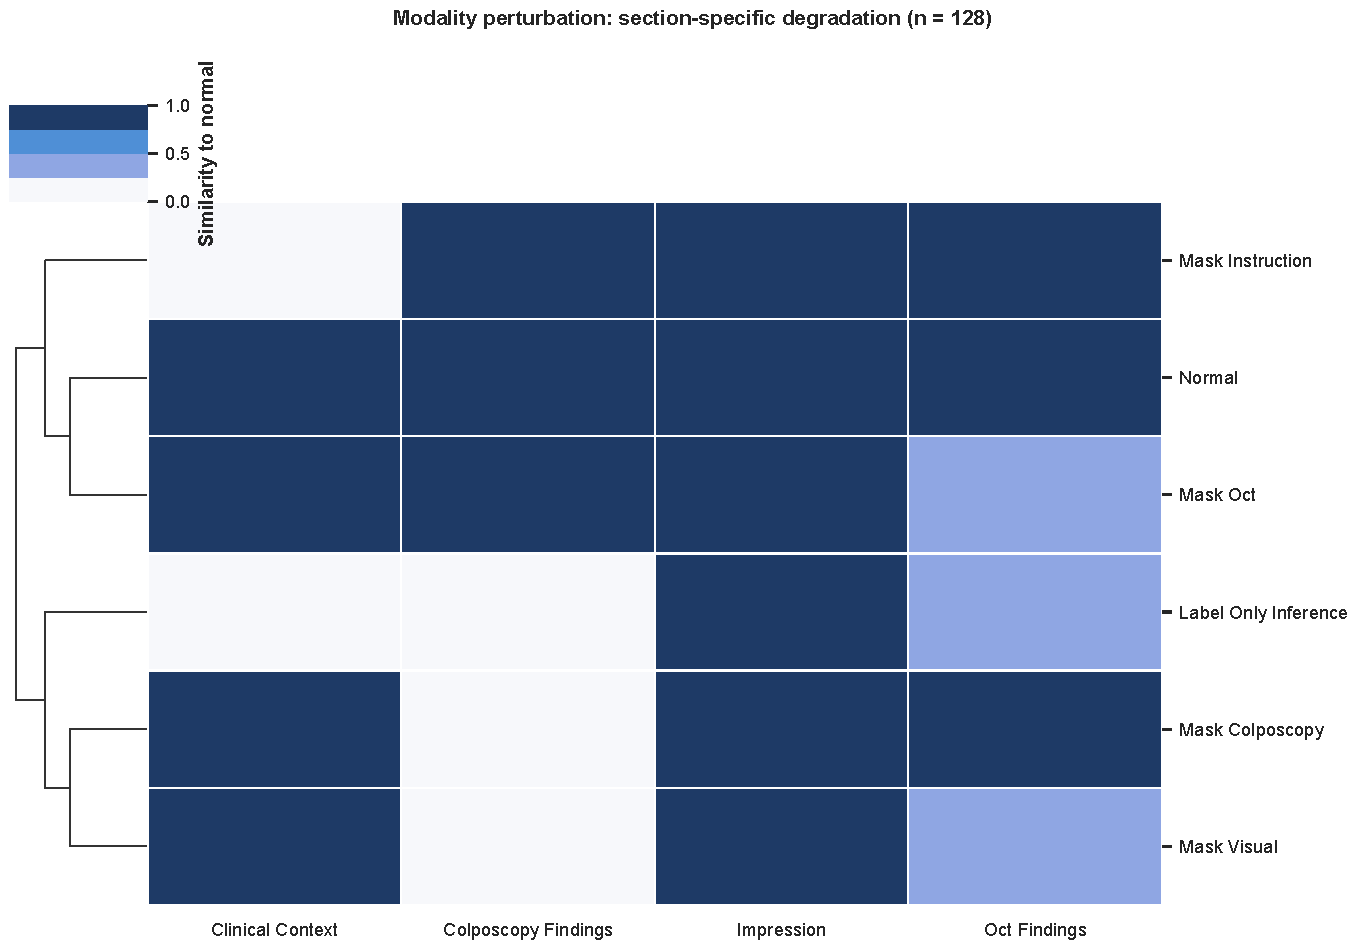
\includegraphics[width=\linewidth]{final_Fig/Figure3_modality_perturbation_heatmap.pdf}
  \caption{Modality perturbation audit. The largest degradation occurs in the report section matched to the perturbed modality, supporting modality-sensitive decoding under the retrospective protocol.}
  \label{fig:perturbation_heatmap}
\end{figure}

\FloatBarrier

\subsection{Centre-level stress tests and robustness constrain generalisation}
\label{subsec:loco_results}

Reference-stratified testing showed that held-out performance was not confined to cases with archived reports: the MOSAIC--RASA backbone achieved AUROC 0.824 among cases with reference reports (\(n=108\)) and AUROC 0.850 among cases without reference reports (\(n=180\)). A stronger strict leave-one-centre-out analysis revealed material centre dependence under fixed quick-budget retraining (Table~\ref{tab:s2_loco_strict_retrain}). Held-out AUROC for the backbone was 0.702 for Enshi, 0.648 for Jingzhou, 0.650 for Shiyan, 0.895 for Wuhan Renmin, and 0.682 for Xiangyang. Eval-only LOCO using a global checkpoint was analysed separately and is not pooled with strict retraining.

\begin{table*}[!htbp]
  \centering
  \caption{Strict leave-one-centre-out retraining under the fixed quick-budget protocol.}
  \label{tab:s2_loco_strict_retrain}
  \scriptsize
  \begin{threeparttable}
  \resizebox{\linewidth}{!}{%
  \begin{tabular}{llrr}
    \toprule
    \textbf{Held-out centre} & \textbf{Model} & \textbf{$n$} & \textbf{AUROC} \\
    \midrule
    Enshi & MOSAIC--RASA backbone & 61 & \textbf{0.702} \\
    Enshi & Real-report-only decoder & 61 & 0.617 \\
    Enshi & Report generation without section alignment & 61 & 0.697 \\
    Jingzhou & MOSAIC--RASA backbone & 55 & 0.648 \\
    Jingzhou & Real-report-only decoder & 55 & 0.615 \\
    Jingzhou & Report generation without section alignment & 55 & \textbf{0.704} \\
    Shiyan & MOSAIC--RASA backbone & 79 & \textbf{0.650} \\
    Shiyan & Real-report-only decoder & 79 & 0.620 \\
    Shiyan & Report generation without section alignment & 79 & 0.640 \\
    Wuhan Renmin & MOSAIC--RASA backbone & 13 & \textbf{0.895} \\
    Wuhan Renmin & Real-report-only decoder & 13 & 0.842 \\
    Wuhan Renmin & Report generation without section alignment & 13 & 0.871 \\
    Xiangyang & MOSAIC--RASA backbone & 80 & \textbf{0.682} \\
    Xiangyang & Real-report-only decoder & 80 & 0.652 \\
    Xiangyang & Report generation without section alignment & 80 & 0.670 \\
    \bottomrule
  \end{tabular}%
  }
  \begin{tablenotes}[flushleft]
    \footnotesize
    \item Strict LOCO is a stress test of centre-held-out retraining, not a definitive external-validation claim.
  \end{tablenotes}
  \end{threeparttable}
\end{table*}

\begin{figure}[!htbp]
  \centering
  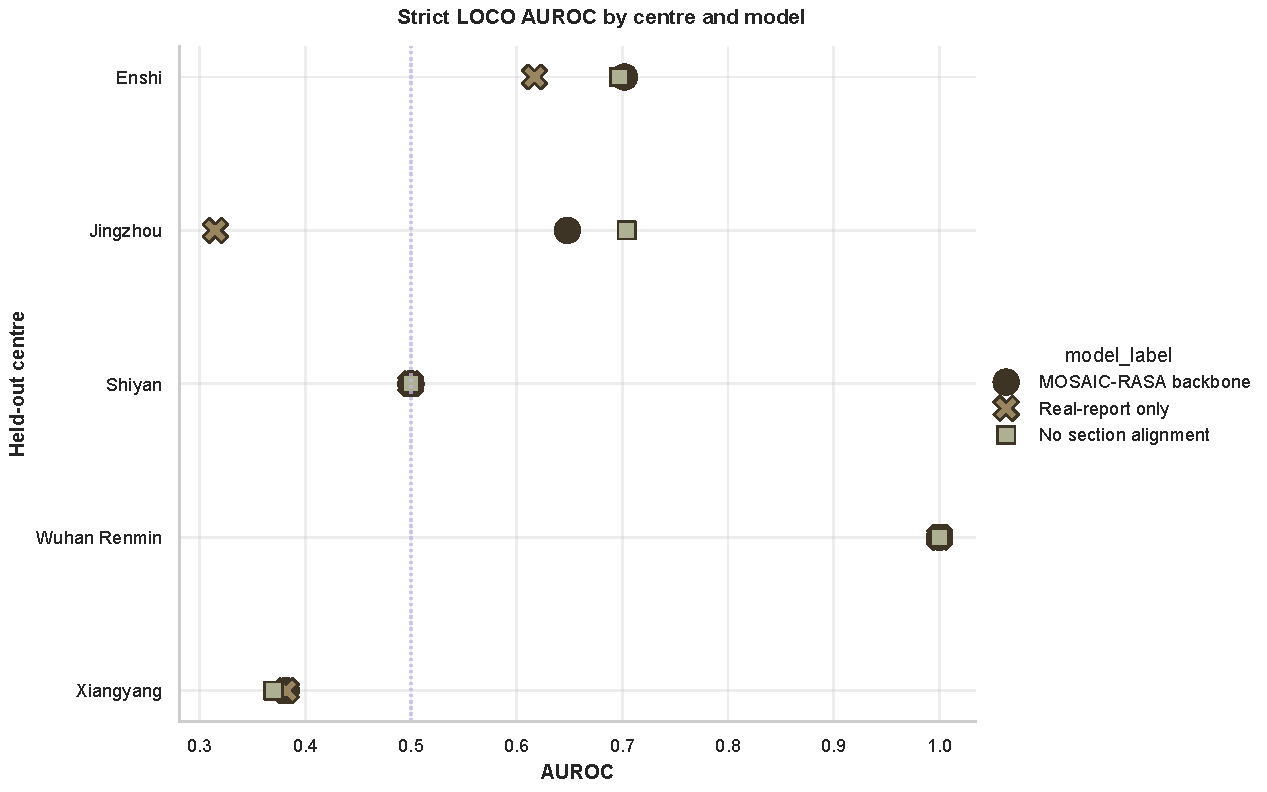
\includegraphics[width=\linewidth]{final_Fig/Figure4_loco_forest_catplot.pdf}
  \caption{Strict leave-one-centre-out behaviour under fixed quick-budget retraining. The centre-wise spread identifies residual distribution shift as a limitation of the current retrospective evidence.}
  \label{fig:loco_heatmap}
\end{figure}

Additional robustness and systems audits supported reproducible retrospective batch analysis while preserving the same claim boundary. Multi-seed AUROC for the MOSAIC--RASA backbone was stable (mean 0.776; 95\% interval, 0.773--0.781; SD 0.004). Report-level safety metrics showed no missing-modality hallucination or section incompleteness in the evaluated settings, with label-report contradiction rate 0.047. The pipeline processed 137,591 images, stored 5,691 embedding files using 47.349 MB, and produced publishable checkpoints of approximately 80 MB. These findings support MOSAIC as a reproducible retrospective semantic-prior analytics framework, while prospective validation, stronger centre-shift mitigation, expert review of generated report sections, and broader foundation-model benchmarking remain necessary before clinical utility can be claimed.

\FloatBarrier

Overall, the evidence chain is internally consistent with the MOSAIC design. The cohort demonstrates incomplete and centre-dependent report supervision; Phase O provides modality-grounded weak-oracle pseudo reports rather than label templates; Phase S improves relative section-wise semantic organisation; report-scarcity analyses show that pseudo-report augmentation is most useful in low-report regimes; and Phase A+I+C improves the locked held-out predictor through train-only semantic retrieval and validation-calibrated fusion. The same evidence also defines the limits of the manuscript: MOSAIC is a retrospective, leakage-controlled semantic-prior learning framework, not an autonomous LLM diagnostic system, not a replacement for clinician-authored reports, and not yet a prospectively validated clinical tool.
